% !TeX TXS-program:compile = txs:///pdflatex/[--shell-escape]

\documentclass[11pt, letterpaper]{article}

\usepackage[utf8]{inputenc}
\usepackage[T1]{fontenc}
\usepackage{lmodern}
\usepackage{graphicx}
\usepackage{longtable}
\usepackage{wrapfig}
\usepackage{rotating}
\usepackage{amsmath}
\usepackage{textcomp}
\usepackage{amssymb}
\usepackage{hyperref}
\usepackage{minted}
\usepackage[spanish]{babel}
\usepackage[round]{natbib}
\usepackage{logicproof}


\title{\textsc{Representación del conocimiento} \\
	Tarea 1
}  

\author{Angel García Báez\\
	Alumno de la Maestría en Inteligencia Artificial \\ \\ \textbf{IIIA}
	Instituto de Investigaciones en Inteligencia Artificial \\
	Universidad Veracruzana \\ \emph{Campus Sur, Calle Paseo Lote II,
		Sección 2a, No 112} \\ \emph{Nuevo Xalapa, Xalapa, Ver., México 91097}
	\\ \\ ZS24019400@estudiantes.uv.mx}

\date{\today}


\begin{document}
	
	
	\maketitle
	
	\section{Cuestionario en Socrative}
	
	Cree una cuenta en https://www.socrative.com para ingresar como \textbf{estudiante} en el salón \textbf{2025RC}. Ahí encontrará un test de opción múltiple a resolver (rc-01). El test puede resolverse en cualquier orden y estará abierto hasta el día de entrega de la tarea. El único medio de entrega es por esta vía. [20/100] \\
	
	El cuestionario de Socrative fue respondido bajo el nombre/alias de \textbf{Angel GB}.
	
	\newpage
	
	\section{Articulo de Yoav Shoham}
	Lea el artículo de Yoav Shoham titulado: "Why Knowledge Representation Matters, A personal story: From philosophy to software". Responda las siguientes preguntas de manera breve y concisa para su discusión en clase.[30/100]
	
	\begin{enumerate}
		\item[a)] ¿En qué sentido la atención que recibe actualmente la IA es diferente de la atención que recibía en los 90s?
		
		\item[b)] De un ejemplo de aplicación donde el enfoque actual de la IA es muy exitoso.
		
		
		\item[c)]  Explique por qué Shoham considera el caso considerado como \textit{filosofía aplicada}.
		
		
		\item[d)] Explique qué significa ese término en el contexto del artículo.
		
		
		\item[e)] ¿Qué significado tiene la abreviatura AGM en el artículo?
		
		
		\item[f)]  Explique en qué consiste el problema de mantenimiento de creencias e intenciones.
		
		\item[g)] ¿Qué es un PTA?
		
		\item[h)] ¿Cuáles son los tres pilares en la construcción de Timeful 1.0?
		
		
		\item[i)] ¿Qué significa que citas, eventos, etc. sean intenciones?
		
		\item[j)] Explique el concepto de IO.
		
		\item[k)] ¿Qué clases de intenciones se consideraban en la versión de 2015?
		
		\item[l)] Explique uno de los mejores ejemplos de como la filosofía influyó las decisiones en el diseño de Timeful.
		
		\item[m)]  ¿De qué manera contribuyó la representación de conocimiento en el desarrollo de Timeful?
		
		\item[n)] ¿Qué problemas hay al querer usar aprendizaje automático en una aplicación como Timeful?
		
		\item[ñ)] ¿Cuál es su conclusión tras la lectura del artículo?
		
	\end{enumerate}
	
	\section{Realizar una demostración}
	
	Pruebe que $\neg p \vee q \vdash p \implies q$. Demuestre que también son sintácticamente equivalentes. [20/100] \\
	
	Para la realización de esta demostración, se hizo uso del conocimiento adquirido durante las clases, así como de las notas largas DEL DR GUERRA a base de prueba y error, como si se intentara armar un rompecabezas, tratando de entender las reglas fundamentales para poder mover las piezas.
	
	\subsection{Primera demostración}
	
	Primero, se hizo la demostración usando la parte izquierda $\neg p \vee q$ para probar que de ahi se sigue $p \implies q$:
	\begin{logicproof}{3}
		\neg p \vee q & premisa \\
		\begin{subproof}
			\neg p & supuesto \\
			\begin{subproof}
				p & supuesto \\
				\bot & contradicción con 2 y 3 \\
				q & (por eliminación de la contradicción 4)
			\end{subproof}
			p \implies q & introducción de la implicación (3-5)
		\end{subproof}
		\begin{subproof}
			q & supuesto \\
			\begin{subproof}
				p & supuesto \\
				q & copia de 7
			\end{subproof}
			p \implies q & por introducción de la implicación de 8 y 9   
		\end{subproof}
		p \implies q & eliminación de la disyunción sobre la premisa 1
	\end{logicproof}
	
	\newpage
	
	\subsection{Segunda demostración}
	
	A continuación se hizo la demostración usando la parte derecha $p \implies q$ para probar que de ahi se sigue $\neg p \vee q$:
	
	\begin{logicproof}{3}
		
		p \implies q & Premisa \\
		p \vee \neg p & Ley del medio excluido (LEM)\\
		\begin{subproof}
			p & Supuesto \\
			q & por Modus Ponens de 1 y 3\\
			\neg p \vee q & Introducción de la disyunción, segunda variante
		\end{subproof}
		\begin{subproof}
			\neg p & Supuesto \\
			\neg p \vee q & Introducción de la disyunción, primera variante
		\end{subproof}
		\neg p \vee q & eliminación de la disyunción sobre la premisa 2
	\end{logicproof}
	
	
	
	\newpage
	
	\section{Inciso 4}
	Descargue el repositorio 
	\begin{center}
		\url{https://github.com/flijnzaad/natural-natural-deduction}    
	\end{center}
	
	que implementa un demostrador de teoremas basado en deducción natural, implementado como una búsqueda en Prolog. Prepare un reporte respondiendo a las siguientes preguntas. Las respuestas se discutirán en clase.
		
	\begin{itemize}
		\item ¿Cómo se representan las preguntas al sistema (\textit{queries})?
		\item ¿Cómo se representan las demostraciones?
		\item De un ejemplo de como funciona el predicado \mintinline{prolog}{connectives/3}. 
		\item ¿Qué hace el predicado \mintinline{prolog}{provesWrap/3}?
		\item ¿Qué tipo de búsqueda implementa el predicado \mintinline{prolog}{provesIDS/7}?
		\item ¿Qué implementa el predicado \mintinline{prolog}{proves/7}?
		\item ¿Cómo se implementa la introducción de la conjunción?
		\item ¿Qué heurística usa la búsqueda de este demostrador?
		\item ¿Donde se implementan las sub-pruebas (cajitas)?
	\end{itemize}
	
	\newpage
	
	\subsection{Reporte}
	
	El programa "Natural" es un demostrador automático basado en las reglas de deducción natural de la lógica. Está implementado en Prolog y cuenta con una interfaz que permite manipular los resultados de las consultas de Prolog desde Python, generando un reporte en formato TeX con los resultados de la demostración. Por defecto, el programa incluye 38 consultas en forma de reglas Prolog, las cuales se utilizan para probar su funcionamiento, realizar las demostraciones y generar el reporte final en formato PDF con Python.
	
	Las consultas implementadas siguen una estructura definida de reglas, donde la cabeza, que es un predicado, toma la variable $X$. Esta construcción se denota mediante el número de la consulta, como $q_1, q_2, \dots , q_n$. El cuerpo de cada regla se compone de tres partes principales: la premisa, que contiene los hechos que queremos probar; la conclusión, que almacena el resultado encontrado; y el predicado \texttt{provesWrap/3}, que se encarga de darle el formato adecuado a la salida.
	
	En el programa, las demostraciones se representan como una lista en la que se van almacenando los pasos válidos que el programa sigue, comenzando con la primera línea de premisa. A medida que avanza, se van construyendo las pruebas y subpruebas necesarias hasta llegar a la conclusión, respetando el índice o número de fila de cada paso, tal como se hace en las demostraciones manuales.	
	
	El programa implementa un predicado llamado connectives/3, cuya tarea es analizar las fórmulas lógicas que se van construyendo para extraer los conectivos (como and, or, not, if, etc.) que aparecen en ellas. Esto resulta especialmente útil, ya que al identificar estos conectivos, el programa puede seleccionar adecuadamente las reglas de inferencia que se deben aplicar según corresponda. Para lograr esto, el predicado utiliza una estructura recursiva por casos, explorando las premisas y conclusiones hasta extraer todos los conectivos y devolver una lista vacía como resultado.
	
	De forma muy simple, si se tienen las premisas $and(p, q)$ y $if(r,s)$ y las conclusiones $or(p,not(s))$, el código debería devolver una lista con los operadores presentes como se muestra en el ejemplo:
	
	\begin{minted}{prolog}
	?- connectives([and(p,q),if(r,s)], or(p,not(s)), L)
	L = [and, if, or, not]
	\end{minted}
	
	
	Por otro lado, el predicado \texttt{provesWrap/3} funciona como una envoltura del predicado principal que se desea demostrar, recopila información sobre los conectivos presentes en las premisas y conclusión, permite estandarizar el flujo de trabajo inicial y delega el trabajo a \texttt{provesWrap/5} que es una versión más completa del predicado que toma en cuenta futuras adiciones a las premisas .
	
	El predicado encargado de construir el árbol de búsqueda en Prolog es \texttt{provesIDS/7}. Este predicado implementa un algoritmo de búsqueda "profunda" (o "deep search") de manera iterativa. Su función es tomar las premisas disponibles y buscar formas lógicas que satisfagan correctamente la demostración. Si no logra encontrar una solución en la profundidad inicial, el algoritmo aumenta gradualmente la profundidad de búsqueda hasta encontrar una demostración válida. Una vez que la encuentra, hace el corte y continúa con el siguiente paso.
	
	Por otro lado, es \texttt{proves/7} el encargado de implementar las reglas de deducción natural que permiten introducir o eliminar elementos de las formulas lógicas de forma recursiva por casos para que \texttt{provesIDS/7} sea el que induzca la búsqueda.
	
	Dentro del abanico de reglas para introducir y eliminar elementos de las formulas, llama la atención la forma en que se implementa la introducción de la conjunción, la regla se fija si ya se ha demostrado $X$ (en la linea $N1$) y $Y$ (en la linea $N2$), si se cumplen ambas condiciones, entonces puede realizar la introducción de la conjunción $X\land Y$ .

	Parece que el demostrador implementa una heurística que busca minimizar la cantidad de líneas necesarias para probar las demostraciones, dado el modo en que se induce el árbol de búsqueda dentro del programa. Esto se evidencia principalmente en la búsqueda IDS, que intenta reducir al mínimo el número de pruebas posibles. Esto se debe a que un aumento excesivo en la profundidad de la búsqueda incrementa el espacio de búsqueda, lo que complica la demostración y aumenta tanto el tiempo como los recursos computacionales necesarios.
	
	Finalmente, las premisas no se demuestran directamente, es necesario ir construyendo sub pruebas que prueban los argumentos a utilizar, para ello, dentro de la lógica del programa se manda a llamar al predicado \texttt{subproof/12} dentro de los casos de la función \texttt{proves/7}.
	
	A modo de probar el potencial de dicho programa, se agrego al archivo de $queries.pl$ la siguiente regla que representa la demostración del inciso 3.2 probado anteriormente a mano:
	
	
	\begin{minted}{prolog}
		q40(X) :-                                    
		Premises = [line(1, or(neg(p), q), premise, 0)],  
		Concl    = line(_, if(p, q), _, _),    
		provesWrap(Premises, Concl, X).		
	\end{minted}

	El resultado arrojado por el programa en formato latex es el siguiente:

	\begin{figure}[h]
		\centering
		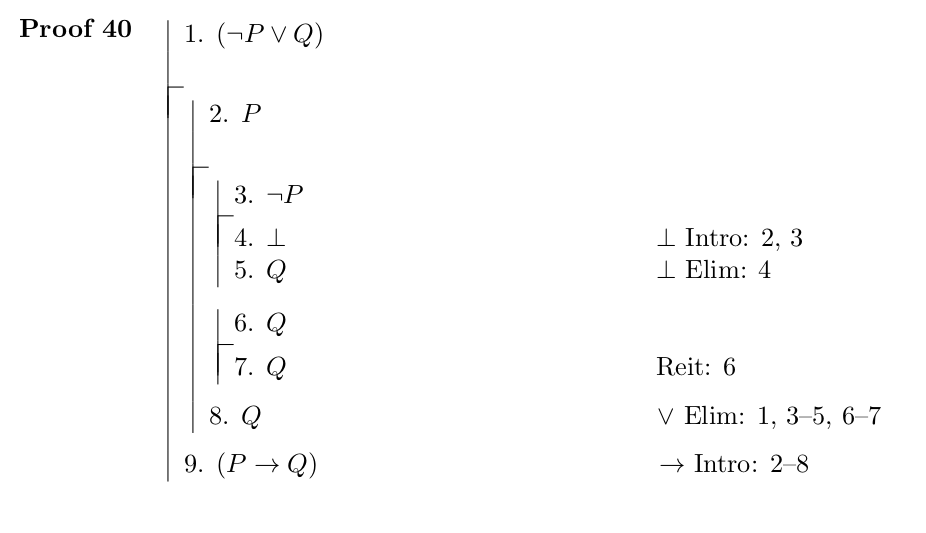
\includegraphics[width=1\textwidth]{IM1.png}  % Ajusta el tamaño y el nombre del archivo
		\caption{Demostración de $\neg P \vee Q \vdash (P \implies Q)$}
		\label{fig:mi_imagen}
	\end{figure}
	
	
	El resultado es prácticamente el mismo, salvo que tiene la notación más formal y bonita.
		
	Es importante señalar que se intentó realizar el complemento de la demostración ($p \implies q$), pero el árbol de búsqueda creció rápidamente, alcanzando una profundidad de 12 sin generar ningún resultado. Se sospecha que, debido a esta limitación, una posible área de mejora del programa sería incorporar la ley del medio excluido, la cual, como se mostró en el inciso 3.1, es fundamental para la correcta resolución de la demostración.
	
	
	\newpage 
	
	REFERENCIAS


	
	
\end{document}


\end{document}
